\section{Ramsey interferometry}

Mach-Zehnder interferometer for atomic internal states.
Consider that pulse 1 is a $\pi/2$ pulse such that:
\begin{align}
    \ket{g}\to\frac{1}{\sqrt{2}}(\ket{e}+\ket{g}).
\end{align}
Say there is a general state-dependent phase shift applied to the states $\ket{g},\ket{e}$ such that 
\begin{align*}
    \frac{1}{\sqrt{2}}(\ket{e}+\ket{g})\to\frac{1}{\sqrt{2}}(\ket{e}+e^{i\phi}\ket{g}).
\end{align*}
Pulse 2 then:
\begin{align*}
    \frac{1}{\sqrt{2}}(\ket{e}+e^{i\phi}\ket{g})\to\frac{1}{\sqrt{2}}[\frac{1}{\sqrt{2}}(\ket{e}-\ket{g})+\frac{e^{i\phi}}{\sqrt{2}}(\ket{e}+\ket{g})]=\frac{1}{2}
    [\ket{e}\underbrace{(1+e^{i\phi})}_{P_e=\frac{1+\cos\phi}{2}}+\ket{g}\underbrace{(1-e^{i\phi})}_{\frac{1-\cos\phi}{2}}]
\end{align*}
For $\phi=0$, $P_e=1$, $P_g=0$ $\{\pi/2+\pi/2=\pi\text{pulse}\}$. The phase $\phi$ depends on possible external field and can be detected by the final 
excitation probability of the atom.
\begin{figure}[htbp]
    \centering
    \begin{subfigure}{.45\columnwidth}
        \centering
        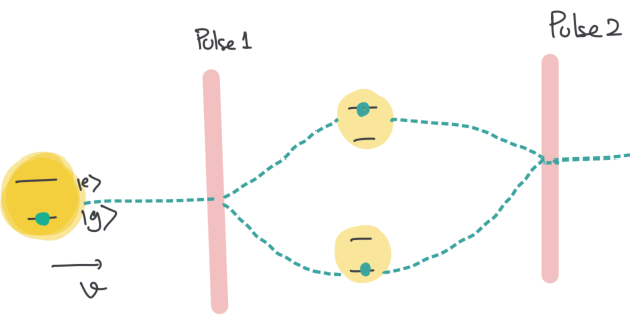
\includegraphics[width=\columnwidth]{PartOne/ChapterFour/figures/ramsey_1.png}
        \caption{Ramsey interferometer}
    \end{subfigure}
    \hfill
    \begin{subfigure}{.4\columnwidth}
        \centering
        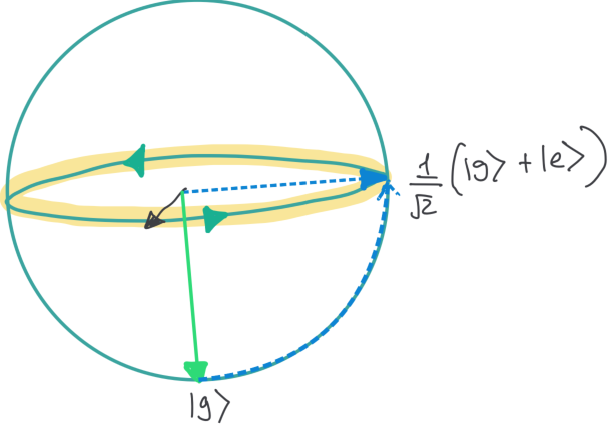
\includegraphics[width=\columnwidth]{PartOne/ChapterFour/figures/ramsey_2.png}
        \caption{Bloch sphere after the $\pi$ pulse}
    \end{subfigure}
\end{figure}
%%
\subsection{Analogy with MZI}
We have:
{\small
\begin{align*}
    \ket{1}_1&=\ha_1^\dagger\ket{0}\\
    &=\frac{\ha_2^\dagger+\ha_3^\dagger}{\sqrt{2}}\ket{0}\\
    \ket{1}_1&=\frac{1}{\sqrt{2}}(\ket{1}_2+\ket{1}_3)\xrightarrow{\pi-\text{pulse}}
    \frac{1}{\sqrt{2}}(\ket{1}_2+e^{i\phi}\ket{1}_3)\xrightarrow{BS}\frac{1}{\sqrt{2}}\left[\frac{\ha^\dagger_4+\ha^\dagger_5}{\sqrt{2}}\ket{0}+e^{i\phi}
    \frac{\ha_4^\dagger-\ha_5^\dagger}{\sqrt{2}}\ket{0}\right]=\frac{1}{2}\left[(1+e^{i\phi})\ket{1}_4+(1-e^{i\phi})\ket{1}_5\right].
\end{align*}}
Probability of detecting a photon at detector D4 and D5 changes with the phase $\phi$.

\begin{figure}[htbp]
    \centering
    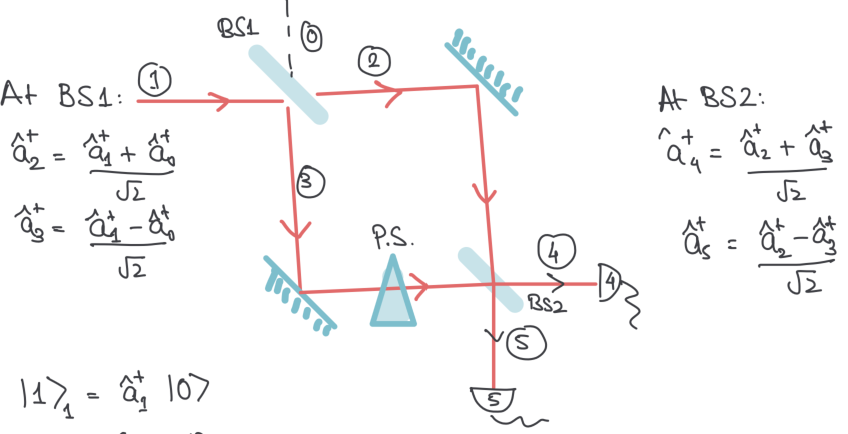
\includegraphics[width=.5\columnwidth]{PartOne/ChapterFour/figures/analogymzi.png}
    \caption{Analogy with MZI.}
\end{figure}